\section{سوال سوم - نظری}

نشان دهید شبکه چند لایه پرسپترونی که فقط از تابع فعال‌سازی \texttt{ReLU} و یا \texttt{pReLU} استفاده می‌کند، تابع پیوسته تکه‌ای خطی می‌سازد.


\begin{qsolve}
از شبکه پرسپترون چند‌لایه می‌توان برای تقریب چند‌جمله ای های مرتبه پایین تکه ای استفاده کرد. \cite{ref1}

دوتا از توابع غیر خطی‌ای که استفاده می‌شود، تابع \lr{ReLU} و \lr{PReLU} است که به صورت زیر تعریف می‌شود:

	\begin{center}
		\includegraphics*[width=0.5\linewidth]{pics/img10.png}
		\captionof{figure}{توابع فعال‌ساز \lr{ReLU} و  \lr{PReLU}}
		\label{توابع فعالساز رلو و پی رلو}
	\end{center}

	$$ r(x)=max(0, x) $$
	
	بنابراین یک تابع تکه ای خطی را می‌توان به صورت زیر نوشت:
	
	$$ f(x)\approx f_l(x)=\sum_{i=0}^{N-1} f(x_i)t_i(x), $$
	$$ \text{where} \qquad t_i(x)=t(h^{-1}(x-x_i)) $$
	
	و تابع $t(x)$ یک تابع مثلثی به صورت زیر است:
	
	$$
	t(x)=
	\begin{cases}
		x+1, \ \ \  \text{if} \ -1\le x \le 0 \\
		-x+1, \ \ \ \text{if} \ 0\le x \le 1 \\
		0,     \ \ \ \text{otherwise.}
	\end{cases}
	$$
	
	با ساختار یک گره در ورودی که $x \in [0,1]$ و یک گره در خروجی که $f(x)$ را می‌سازد می‌توان یک شبکه \lr{MLP} که متشکل از ۳ لایه (ورودی + مخفی + خروجی) و ۴ نرون وروی است به صورت زیر پیشنهاد داد:
	
	$$ R_{in} \rightarrow R_{j, 1}: \alpha_{j, 1}=h^{-1}, \xi_{j,1}=-h^{-1}x_{j-1} $$ \\
	$$ R_{in} \rightarrow R_{j, 2}: \alpha_{j, 2}=h^{-1}, \xi_{j,2}=-h^{-1}x_{j} $$ \\
	$$ R_{in} \rightarrow R_{j, 3}: \alpha_{j, 3}=h^{-1}, \xi_{j,3}=-h^{-1}x_{j+1} $$ \\
	$$ R_{in} \rightarrow R_{j, 4}: \alpha_{j, 4}=h^{-1}, \xi_{j,4}=-h^{-1}x_{j} $$ \\
	
\end{qsolve}




\begin{qsolve}
	در شکل‌های زیر خروجی نرون‌های شبکه پس از عبور از تابع فعال‌سازی \lr{R آورده شده است:
		
		\begin{figure}
			\centering
			\begin{subfigure}{0.4\textwidth}
				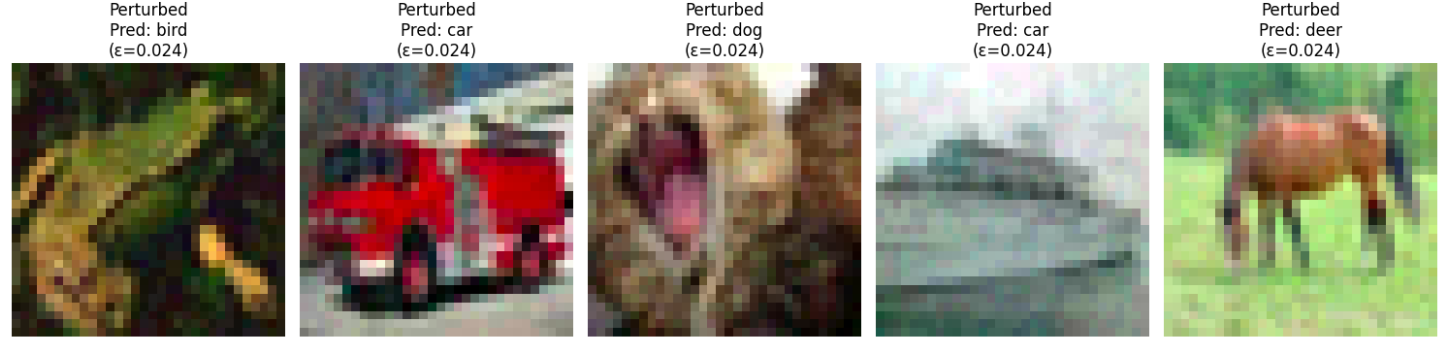
\includegraphics[width=\textwidth]{img11}
				\caption{Firts subfigure.}
				\label{fig:first}
			\end{subfigure}
			\hfill
			\begin{subfigure}{0.4\textwidth}
				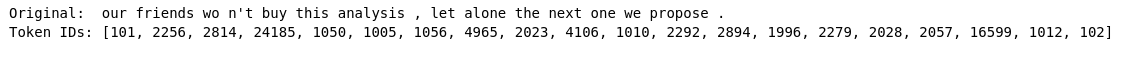
\includegraphics[width=\textwidth]{img12}
				\caption{Second subfigure.}
				\label{fig:second}
			\end{subfigure}
			\hfill
		\end{figure}
\end{qsolve}












\begin{latin}
	\begin{thebibliography}{9}
		\bibitem{ref1}
		Lin R, You S, Rao R, Kuo CC. Constructing multilayer perceptrons as piecewise low-order polynomial approximators: a signal processing approach. arXiv preprint arXiv:2010.07871. 2020 Oct 15.	
	\end{thebibliography} 
\end{latin}










%فرض کنید می‌خواهیم تابع $f(x)=sin(x)+3x^{17}-5x^2$ را با یک نورون پرسپترونی تخمین و درصورت امکان محاسبه نماییم.
%
%\begin{enumerate}
%	\item با تحقیق و مطالعه کافی توضیح دهید چگونه می‌توان از سری تیلور برای تخمین توابع استفاده نمود؟
%	
%	\begin{qsolve}
%		سری تیلور بیان می‌کند که ما می‌توانیم هر تابع $n$ بار مشتق‌پذیری را بر اساس یک مجموع بی‌نهایت از مشتق‌های آن حول نقطه صفر بنویسیم. فرمول بسط تیلور به صورت زیر بیان می‌شود:
%		
%		$$
%		\sum_{n=0}^{\infty} \frac{f^{(n)}(0)}{n!}(x)^n=f(0)+\frac{f'(0)}{1!}(x)+\frac{f''(0)}{2!}(x)^2+...+\frac{f^{(n)}(0)}{n!}(x)^n
%		$$
%		
%		آقای مکلورن این تقریب را به صورت عمومی گسترش داد و بیان کرد که می‌توان توابع مختلف $n$ بار  مشتق‌پذیر را حول هر نقطع مشخصی بسط داد و فرمول تیلور را به صورت زیر بازنویسی کرد:
%		
%		
%		$$
%		\sum_{n=0}^{\infty} \frac{f^{(n)}(a)}{n!}(x-a)^n=f(a)+\frac{f'(a)}{1!}(x-a)+\frac{f''(a)}{2!}(x-a)^2+...+\frac{f^{(n)}(a)}{n!}(x-a)^n
%		$$
%		
%		بنابر این هر تابع $n$ بار مشتق‌پذیری را با داشتن مشتق‌های آن و مقدار آن تابع در نقطه مورد نظر، تقریب زد. برای مثال، تابع $e^x$، $n$ بارمشتق‌پذیر است پس می‌توان نوشت:
%		
%		\begin{eqnarray*}
%			 f(x)&=&e^x \rightarrow f'(x)=f''(x)=f'''(x)=f^{(4)}(x)=...=f^{(n)}(x)=e^x\\
%			 if\quad a&=&0 \rightarrow e^x \approx e^0 + \frac{e^0}{1!}(x) + \frac{e^0}{2!}(x)^2+\frac{e^0}{3!}(x)^3+...+\frac{e^0}{n!}(x)^n\\
%			 &=& 1+x+\frac{1}{2}x^2+\frac{1}{6}x^3+...+\frac{1}{n!}x^n=\sum_{0}^{\infty}\frac{1}{n!}x^n
%		\end{eqnarray*}
%		
%		طبیعتا هرچقدر تعداد جملات بیشتری را در مجموع باهم جمع کنیم، تقریب دقیق تری از تابع حاصل می‌شود اما بار محاسباتی سنگین تر می‌شود و نیازمند محاسبه مشتق‌هایی با مرتبه‌های بالا هستیم.
%	\end{qsolve}
%	
%	
%	
%	
%	\item با استتفاده از سری تیلور، تخمین تابع یاد شده را تا ۱۰ جمله محاسبه و بدست آورید. فرایند محاسبه را در گزارش بنویسید.
%	
%	\begin{qsolve}
%		تابع داده شده از ۲ ترم تشکیل شده است. ترمی سینوسی و ترم چند‌جمله ای. به دلیل آنکه از چند‌جمله ای تبلور استفاده می‌کنیم برای تقریب و $a=0$ است، مقادیر این ترم و مشتقات آن در نقطه صفر، صفر خواهد بود. بنابر این این دو ترم چند جمله ای را که در پایین با آبی مشخص شده است را با تقریب تیلور محاسبه نمی‌کنیم و فقط ترم سینوسی را با استفاده از سری تیلور حساب می‌کنیم. مشتقات تابع سینوسی (تا مرتبه ۹) رامحاسبه می‌کنیم و مقادیر آنها در نقطه صفر محاسبه کرده و آن‌ها را در فرمول سری تیلور قرار می‌دهیم. درنهایت ترم چند جمله ای را عینا به تابع تقریب زده شده اضاف می‌کنیم. محاسبات را به صورت زیر انجام داده ایم:
%	\end{qsolve}
%	
%	\begin{qsolve}
%		\begin{eqnarray*}
%			f(x)&=&sin(x)+3x^{17}-5x^2\\
%			f_1(x)&=&sin(x): a=0 \rightarrow \sum_{0}^{9} \frac{f_1^{(n)}(0)}{n!}x^n=f_1(0)+\frac{f'_1(0)}{1!}x^1+...+\frac{f_1^{(9)}(0)}{9!}x^9\\
%			f_1(x)&=&sin(x) \rightarrow f_1(0)=0\\
%			f'_1(x)&=&cos(x) \rightarrow f'_1(0)=1\\
%			f''_1(x)&=&-sin(x) \rightarrow f''_1(0)=0\\
%			f'''_1(x)&=&-cos(x) \rightarrow f''_1(0)=-1\\
%			f_1^{(4)}(x)&=&sin(x) \rightarrow f_1^{(4)}(0)=0\\
%			&.&\\
%			&.&\\
%			&.&\\
%			f_1^{(9)}(x)&=&cos(x) \rightarrow f_1^{(9)}(0)=1\\
%			\rightarrow &=& 0 + \frac{1}{1!}x^1+\frac{0}{2!}x^2+\frac{-1}{3!}x^3+\frac{0}{4!}x^4+\frac{1}{5!}x^5+\frac{0}{6!}x^6+\frac{-1}{7!}x^7+\frac{0}{8!}x^8+\frac{1}{9!}x^9\\
%			&=& x-\frac{1}{6}x^3+\textcolor{blue}{\frac{1}{120}x^5}-\frac{1}{5040}x^7+\textcolor{blue}{\frac{1}{362880}x^9}=\hat{f(x)}
%		\end{eqnarray*}
%		
%برای آنکه بتوانیم تمام ترم های تابع را رسم نماییم، آن را به صورت زیر می‌نویسیم:
%
%		\begin{eqnarray*}
%			f(x)&=&p_1(x)+p_2(x)+p_3(x)\\
%			p_1(x)&=&sin(x)=x-\frac{1}{6}x^3+\frac{1}{120}x^5-\frac{1}{5040}x^7+\frac{1}{362880}x^9\\
%			p_2(x)&=&3x^{17}\\
%			p_3(x)&=&-5x^2
%		\end{eqnarray*}
%		
%		با فرمت نوشته شده توابه را رسم می‌کنیم. $p_2(x)$ و $p_3(3)$ به‌صورت زیر است:
%		
%		\begin{center}
%			\includegraphics*[width=1\linewidth]{pics/img18.png}
%			\captionof{figure}{ترم‌های چند جمله‌ای تابع}
%			\label{ترم‌های چند جمله‌ای تابع}
%		\end{center}
%	\end{qsolve}
%	
%	
%	\begin{qsolve}
%		ترم سینوسی اصلی و سینوسی تقریب زده شده با سری تیلور به صورت زیر گزارش می‌شود:
%		
%		\begin{center}
%			\includegraphics*[width=1\linewidth]{pics/img19.png}
%			\captionof{figure}{ترم سینوسی اصلی و تقریب زده شده}
%			\label{ترم سینوسی اصلی و تقریب زده شده}
%		\end{center}
%		
%		در نهایت تابع $f(x)$ و تابعی که با ۱۰ جمله از سری تبلور تقریب زده ایم ($\hat{f(x)}$) به صورت زیر گزارش می‌شود:
%		
%		\begin{center}
%			\includegraphics*[width=1\linewidth]{pics/img20.png}
%			\captionof{figure}{تابع اصلی و تابع تقریب زده شده}
%			\label{تابع اصلی و تابع تقریب زده شده}
%		\end{center}
%		
%		
%		
%		
%		
%	\end{qsolve}
%	
%	
%	\item حال یک نرون پرسپترونی طراحی نمایید که بتواند تابع فوق را با جملات سری تیلور محاسبه کند (وزن‌های نورون را با محاسبات بدست‌آورده و در گزارش خود بیان کنید.)
%	در یک نمودار، تابع و تخمین‌های آن را به ازای استفاده از جملات ۱ تا ۱۰ رسم کنید (خروجی ۱۱ منهنی خواهد بود). در یک جدول خطای حاصل از تقریب را به ازای استفاده از جملات مختلف با تابع MSE گزارش کنید.
%\end{enumerate}
%
%\textbf{توجه مهم:‌ ورودی نورون‌های طراحی شده‌تان صرفا بایستی توانی از ویژگی‌های اصلی یا حاصل ضرب توانی از ویژگی‌ها باشد و فرم دیگری قابل قبول نیست. برای مثال اگر یک ویژگی $x$ باشد، $sin(x)$ یا $e^x$ نمی‌تواند ورودی یک نورون باشد.}
%
%\begin{qsolve}
%	حقیقتا بنده این قسمت را دقیق متوجه نشدم. به همین دلیل از نوشتن این قسمت خودداری کردم.
%\end{qsolve}